% Comparative flows: existing TinyML baselines vs Hybrid-in-TA
% Compile: pdflatex tee_qai_baseline_comparison.tex
% Companion to: tee_qai_edge_architecture.tex (Page 3 budget figures)
%
% CHANGELOG
% [2025-06-21] Added reference citations for Rows A/B/C, datasets, OP-TEE,
%   QML prior work, and cost-metric standards (Page 4).
\documentclass[tikz,border=10pt]{standalone}
\usepackage[T1]{fontenc}
\usepackage{lmodern}
\usepackage{xcolor}
\usepackage{url}
\usepackage{tikz}
\usetikzlibrary{arrows.meta,calc,positioning,fit}

\definecolor{zoneoffline}{HTML}{FFE0B2}
\definecolor{zoneedge}{HTML}{E0E0E0}
\definecolor{zoneree}{HTML}{FFCDD2}
\definecolor{zonetee}{HTML}{BBDEFB}
\definecolor{zonecloud}{HTML}{B3E5FC}

\definecolor{filloffline}{HTML}{FFE0B2}
\definecolor{fillree}{HTML}{FFCDD2}
\definecolor{filltee}{HTML}{BBDEFB}
\definecolor{fillcloud}{HTML}{B3E5FC}
\definecolor{filliot}{HTML}{C8E6C9}

\tikzset{
  cmp/.style={draw=black!65, rounded corners=3pt, line width=0.7pt, fill=white,
    align=center, inner sep=4pt, minimum height=0.65cm, font=\small},
  zone/.style={draw=black!55, rounded corners=5pt, line width=0.85pt, inner sep=8pt, opacity=0.35},
  arr/.style={-{Latex}, line width=0.85pt, draw=black!70},
  trust/.style={-{Latex}, line width=0.9pt, draw=blue!60!black},
  deploy/.style={-{Latex}, line width=0.85pt, draw=orange!70!black, dashed},
  lbl/.style={font=\scriptsize, fill=white, inner sep=1pt, text=black!70},
  notebox/.style={draw=black!35, rounded corners=3pt, fill=white, font=\scriptsize,
    align=left, inner sep=5pt, text width=4.2cm},
  rowtitle/.style={font=\bfseries\normalsize, anchor=west},
  figtitle/.style={font=\bfseries\large, align=center, text width=0.95\linewidth},
  figsubtitle/.style={font=\small, align=center, text=black!65, text width=0.95\linewidth},
  qpage/.style={anchor=north west, align=left, text width=16.8cm, inner sep=0pt, font=\footnotesize},
}

\newcommand{\qaheading}[1]{\par\vspace{6pt}{\bfseries\normalsize #1}\par\vspace{3pt}}

\begin{document}
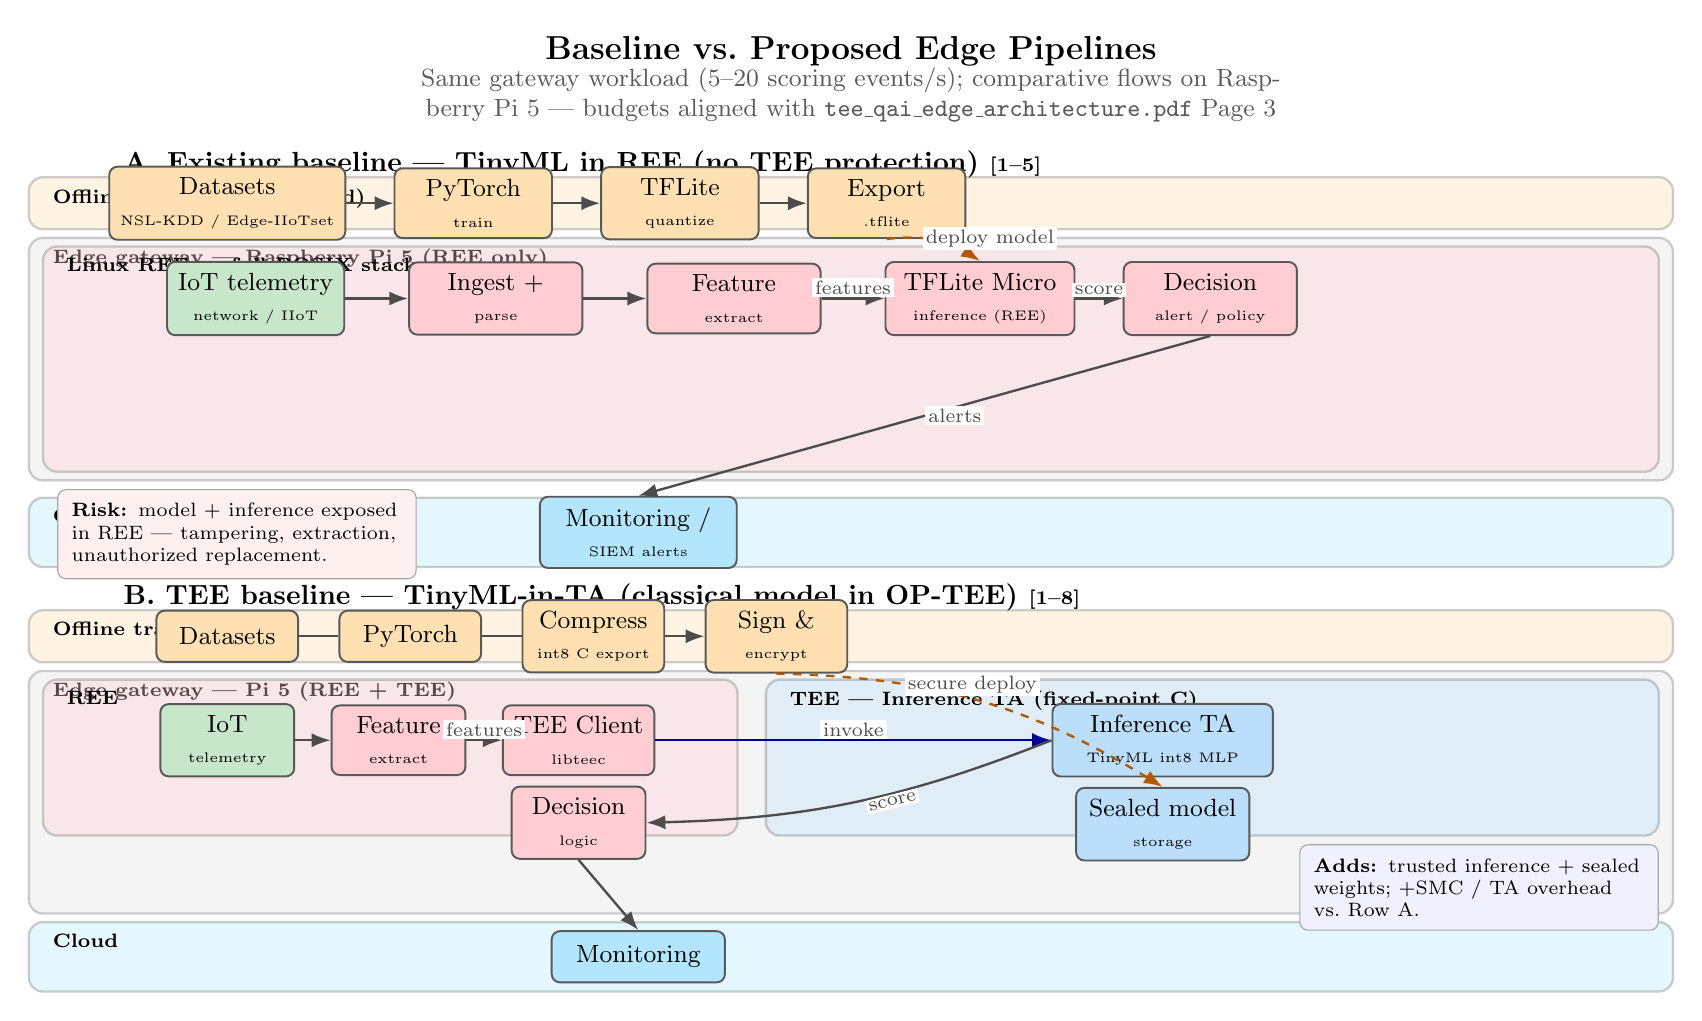
\begin{tikzpicture}[x=18.0cm, y=11.0cm]

\node[figtitle] at (0.50, 1.05) {Baseline vs.\ Proposed Edge Pipelines};
\node[figsubtitle] at (0.50, 1.00) {Same gateway workload (5--20 scoring events/s); comparative flows on Raspberry Pi~5 --- budgets aligned with \texttt{tee\_qai\_edge\_architecture.pdf} Page~3};

%% =====================================================================
%% Row A — Existing: TinyML in REE only (no TEE)
%% =====================================================================
\node[rowtitle] at (-0.02, 0.92) {A.\ Existing baseline --- TinyML in REE (no TEE protection) {\scriptsize [1--5]}};

\draw[zone, fill=zoneoffline] (-0.08, 0.845) rectangle (1.08, 0.905);
\node[anchor=north west, font=\bfseries\scriptsize] at (-0.07, 0.903) {Offline training (host/cloud)};

\draw[zone, fill=zoneedge] (-0.08, 0.555) rectangle (1.08, 0.835);
\node[anchor=north west, font=\bfseries\scriptsize] at (-0.07, 0.833) {Edge gateway --- Raspberry Pi~5 (REE only)};

\draw[zone, fill=zoneree] (-0.07, 0.565) rectangle (1.07, 0.825);
\node[anchor=north west, font=\bfseries\scriptsize] at (-0.06, 0.823) {Linux REE --- full POSIX stack};

\draw[zone, fill=zonecloud] (-0.08, 0.455) rectangle (1.08, 0.535);
\node[anchor=north west, font=\bfseries\scriptsize] at (-0.07, 0.533) {Cloud monitoring};

\node[cmp, fill=filloffline, minimum width=2.0cm] (a_ds) at (0.06, 0.875) {Datasets\\{\tiny NSL-KDD / Edge-IIoTset}};
\node[cmp, fill=filloffline, minimum width=2.0cm, right=0.6cm of a_ds] (a_pt) {PyTorch\\{\tiny train}};
\node[cmp, fill=filloffline, minimum width=2.0cm, right=0.6cm of a_pt] (a_tfl) {TFLite\\{\tiny quantize}};
\node[cmp, fill=filloffline, minimum width=2.0cm, right=0.6cm of a_tfl] (a_exp) {Export\\{\tiny .tflite}};

\node[cmp, fill=filliot, minimum width=2.2cm] (a_iot) at (0.08, 0.765) {IoT telemetry\\{\tiny network / IIoT}};
\node[cmp, fill=fillree, minimum width=2.2cm, right=0.8cm of a_iot] (a_ing) {Ingest +\\{\tiny parse}};
\node[cmp, fill=fillree, minimum width=2.2cm, right=0.8cm of a_ing] (a_feat) {Feature\\{\tiny extract}};
\node[cmp, fill=fillree, minimum width=2.4cm, right=0.8cm of a_feat] (a_inf) {TFLite Micro\\{\tiny inference (REE)}};
\node[cmp, fill=fillree, minimum width=2.2cm, right=0.6cm of a_inf] (a_dec) {Decision\\{\tiny alert / policy}};

\node[cmp, fill=fillcloud, minimum width=2.5cm] (a_mon) at (0.35, 0.495) {Monitoring /\\{\tiny SIEM alerts}};

\draw[arr] (a_ds) -- (a_pt);
\draw[arr] (a_pt) -- (a_tfl);
\draw[arr] (a_tfl) -- (a_exp);
\draw[deploy, dashed] (a_exp.south) to[bend left=20] node[lbl, pos=0.35, right] {deploy model} (a_inf.north);
\draw[arr] (a_iot) -- (a_ing);
\draw[arr] (a_ing) -- (a_feat);
\draw[arr] (a_feat) -- node[lbl, above] {features} (a_inf);
\draw[arr] (a_inf) -- node[lbl, above] {score} (a_dec);
\draw[arr] (a_dec.south) -- node[lbl, right] {alerts} (a_mon.north);

\node[notebox, fill=red!6, anchor=north west] at (-0.06, 0.545) {%
  \textbf{Risk:} model + inference exposed in REE --- tampering, extraction, unauthorized replacement.};

%% =====================================================================
%% Row B — TEE baseline: TinyML-in-TA (same model, protected)
%% =====================================================================
\node[rowtitle] at (-0.02, 0.42) {B.\ TEE baseline --- TinyML-in-TA (classical model in OP-TEE) {\scriptsize [1--8]}};

\draw[zone, fill=zoneoffline] (-0.08, 0.345) rectangle (1.08, 0.405);
\node[anchor=north west, font=\bfseries\scriptsize] at (-0.07, 0.403) {Offline training};

\draw[zone, fill=zoneedge] (-0.08, 0.055) rectangle (1.08, 0.335);
\node[anchor=north west, font=\bfseries\scriptsize] at (-0.07, 0.333) {Edge gateway --- Pi~5 (REE + TEE)};

\draw[zone, fill=zoneree] (-0.07, 0.145) rectangle (0.42, 0.325);
\node[anchor=north west, font=\bfseries\scriptsize] at (-0.06, 0.323) {REE};

\draw[zone, fill=zonetee] (0.44, 0.145) rectangle (1.07, 0.325);
\node[anchor=north west, font=\bfseries\scriptsize] at (0.45, 0.323) {TEE --- Inference TA (fixed-point C)};

\draw[zone, fill=zonecloud] (-0.08, -0.035) rectangle (1.08, 0.045);
\node[anchor=north west, font=\bfseries\scriptsize] at (-0.07, 0.043) {Cloud};

\node[cmp, fill=filloffline, minimum width=1.8cm] (b_ds) at (0.06, 0.375) {Datasets};
\node[cmp, fill=filloffline, minimum width=1.8cm, right=0.5cm of b_ds] (b_pt) {PyTorch};
\node[cmp, fill=filloffline, minimum width=1.8cm, right=0.5cm of b_pt] (b_cmp) {Compress\\{\tiny int8 C export}};
\node[cmp, fill=filloffline, minimum width=1.8cm, right=0.5cm of b_cmp] (b_sig) {Sign \&\\{\tiny encrypt}};

\node[cmp, fill=filliot, minimum width=1.7cm] (b_iot) at (0.06, 0.255) {IoT\\{\tiny telemetry}};
\node[cmp, fill=fillree, minimum width=1.7cm, right=0.45cm of b_iot] (b_feat) {Feature\\{\tiny extract}};
\node[cmp, fill=fillree, minimum width=1.7cm, right=0.45cm of b_feat] (b_tee) {TEE Client\\{\tiny libteec}};
\node[cmp, fill=fillree, minimum width=1.7cm, below=0.12cm of b_tee] (b_dec) {Decision\\{\tiny logic}};

\node[cmp, fill=filltee, minimum width=2.8cm] (b_ta) at (0.72, 0.255) {Inference TA\\{\tiny TinyML int8 MLP}};
\node[cmp, fill=filltee, minimum width=2.2cm, below=0.12cm of b_ta] (b_store) {Sealed model\\{\tiny storage}};

\node[cmp, fill=fillcloud, minimum width=2.2cm] (b_mon) at (0.35, 0.005) {Monitoring};

\draw[arr] (b_ds) -- (b_pt) -- (b_cmp) -- (b_sig);
\draw[deploy, dashed] (b_sig.south) to[bend left=15] node[lbl, pos=0.3, right] {secure deploy} (b_store.north);
\draw[arr] (b_iot) -- (b_feat);
\draw[arr] (b_feat) -- node[lbl, above, sloped] {features} (b_tee);
\draw[trust] (b_tee.east) -- node[lbl, above] {invoke} (b_ta.west);
\draw[arr] (b_ta.west) to[bend left=10] node[lbl, pos=0.4, below, sloped] {score} (b_dec.east);
\draw[arr] (b_dec.south) -- (b_mon.north);

\node[notebox, fill=blue!6, anchor=north east] at (1.07, 0.135) {%
  \textbf{Adds:} trusted inference + sealed weights; +SMC / TA overhead vs.\ Row A.};

\end{tikzpicture}

\newpage
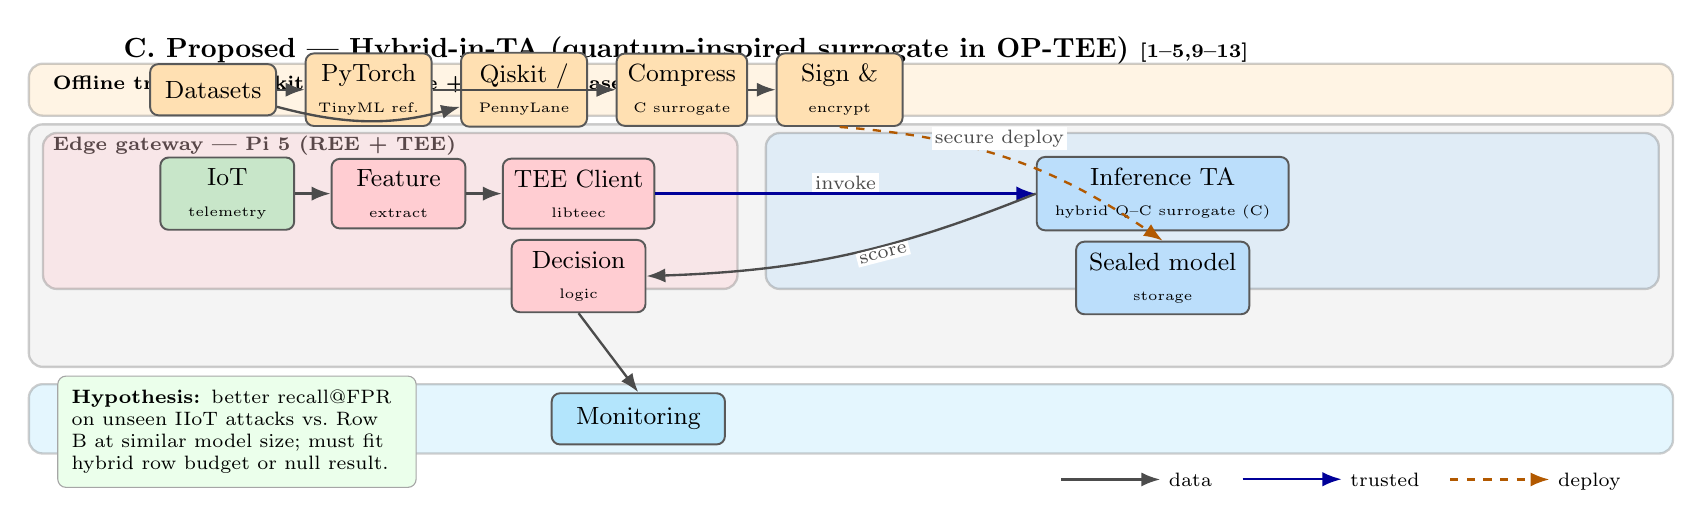
\begin{tikzpicture}[x=18.0cm, y=11.0cm]

\node[rowtitle] at (-0.02, 0.98) {C.\ Proposed --- Hybrid-in-TA (quantum-inspired surrogate in OP-TEE) {\scriptsize [1--5,9--13]}};

\draw[zone, fill=zoneoffline] (-0.08, 0.905) rectangle (1.08, 0.965);
\node[anchor=north west, font=\bfseries\scriptsize] at (-0.07, 0.963) {Offline training (Qiskit/PennyLane + PyTorch baseline)};

\draw[zone, fill=zoneedge] (-0.08, 0.615) rectangle (1.08, 0.895);
\node[anchor=north west, font=\bfseries\scriptsize] at (-0.07, 0.893) {Edge gateway --- Pi~5 (REE + TEE)};

\draw[zone, fill=zoneree] (-0.07, 0.705) rectangle (0.42, 0.885);
\draw[zone, fill=zonetee] (0.44, 0.705) rectangle (1.07, 0.885);

\draw[zone, fill=zonecloud] (-0.08, 0.515) rectangle (1.08, 0.595);

\node[cmp, fill=filloffline, minimum width=1.6cm] (c_ds) at (0.05, 0.935) {Datasets};
\node[cmp, fill=filloffline, minimum width=1.6cm, right=0.35cm of c_ds] (c_pt) {PyTorch\\{\tiny TinyML ref.}};
\node[cmp, fill=filloffline, minimum width=1.6cm, right=0.35cm of c_pt] (c_qk) {Qiskit /\\{\tiny PennyLane}};
\node[cmp, fill=filloffline, minimum width=1.6cm, right=0.35cm of c_qk] (c_cmp) {Compress\\{\tiny C surrogate}};
\node[cmp, fill=filloffline, minimum width=1.6cm, right=0.35cm of c_cmp] (c_sig) {Sign \&\\{\tiny encrypt}};

\node[cmp, fill=filliot, minimum width=1.7cm] (c_iot) at (0.06, 0.815) {IoT\\{\tiny telemetry}};
\node[cmp, fill=fillree, minimum width=1.7cm, right=0.45cm of c_iot] (c_feat) {Feature\\{\tiny extract}};
\node[cmp, fill=fillree, minimum width=1.7cm, right=0.45cm of c_feat] (c_tee) {TEE Client\\{\tiny libteec}};
\node[cmp, fill=fillree, minimum width=1.7cm, below=0.12cm of c_tee] (c_dec) {Decision\\{\tiny logic}};

\node[cmp, fill=filltee, minimum width=3.2cm] (c_ta) at (0.72, 0.815) {Inference TA\\{\tiny hybrid Q--C surrogate (C)}};
\node[cmp, fill=filltee, minimum width=2.2cm, below=0.12cm of c_ta] (c_store) {Sealed model\\{\tiny storage}};

\node[cmp, fill=fillcloud, minimum width=2.2cm] (c_mon) at (0.35, 0.555) {Monitoring};

\draw[arr] (c_ds) -- (c_pt);
\draw[arr] (c_ds) to[bend right=15] (c_qk);
\draw[arr] (c_pt) -- (c_cmp);
\draw[arr] (c_qk) -- (c_cmp);
\draw[arr] (c_cmp) -- (c_sig);
\draw[deploy, dashed] (c_sig.south) to[bend left=15] node[lbl, pos=0.25, right] {secure deploy} (c_store.north);
\draw[arr] (c_iot) -- (c_feat);
\draw[arr] (c_feat) -- (c_tee);
\draw[trust] (c_tee.east) -- node[lbl, above] {invoke} (c_ta.west);
\draw[arr] (c_ta.west) to[bend left=10] node[lbl, pos=0.4, below, sloped] {score} (c_dec.east);
\draw[arr] (c_dec.south) -- (c_mon.north);

\node[notebox, fill=green!8, anchor=north west] at (-0.06, 0.605) {%
  \textbf{Hypothesis:} better recall@FPR on unseen IIoT attacks vs.\ Row B at similar model size; must fit hybrid row budget or null result.};

\node[font=\scriptsize, anchor=north east] at (1.05, 0.505) {%
  \tikz{\draw[arr] (0,0)--(0.07,0);} data \quad
  \tikz{\draw[trust] (0,0)--(0.07,0);} trusted \quad
  \tikz{\draw[deploy] (0,0)--(0.07,0);} deploy};

\end{tikzpicture}

\newpage
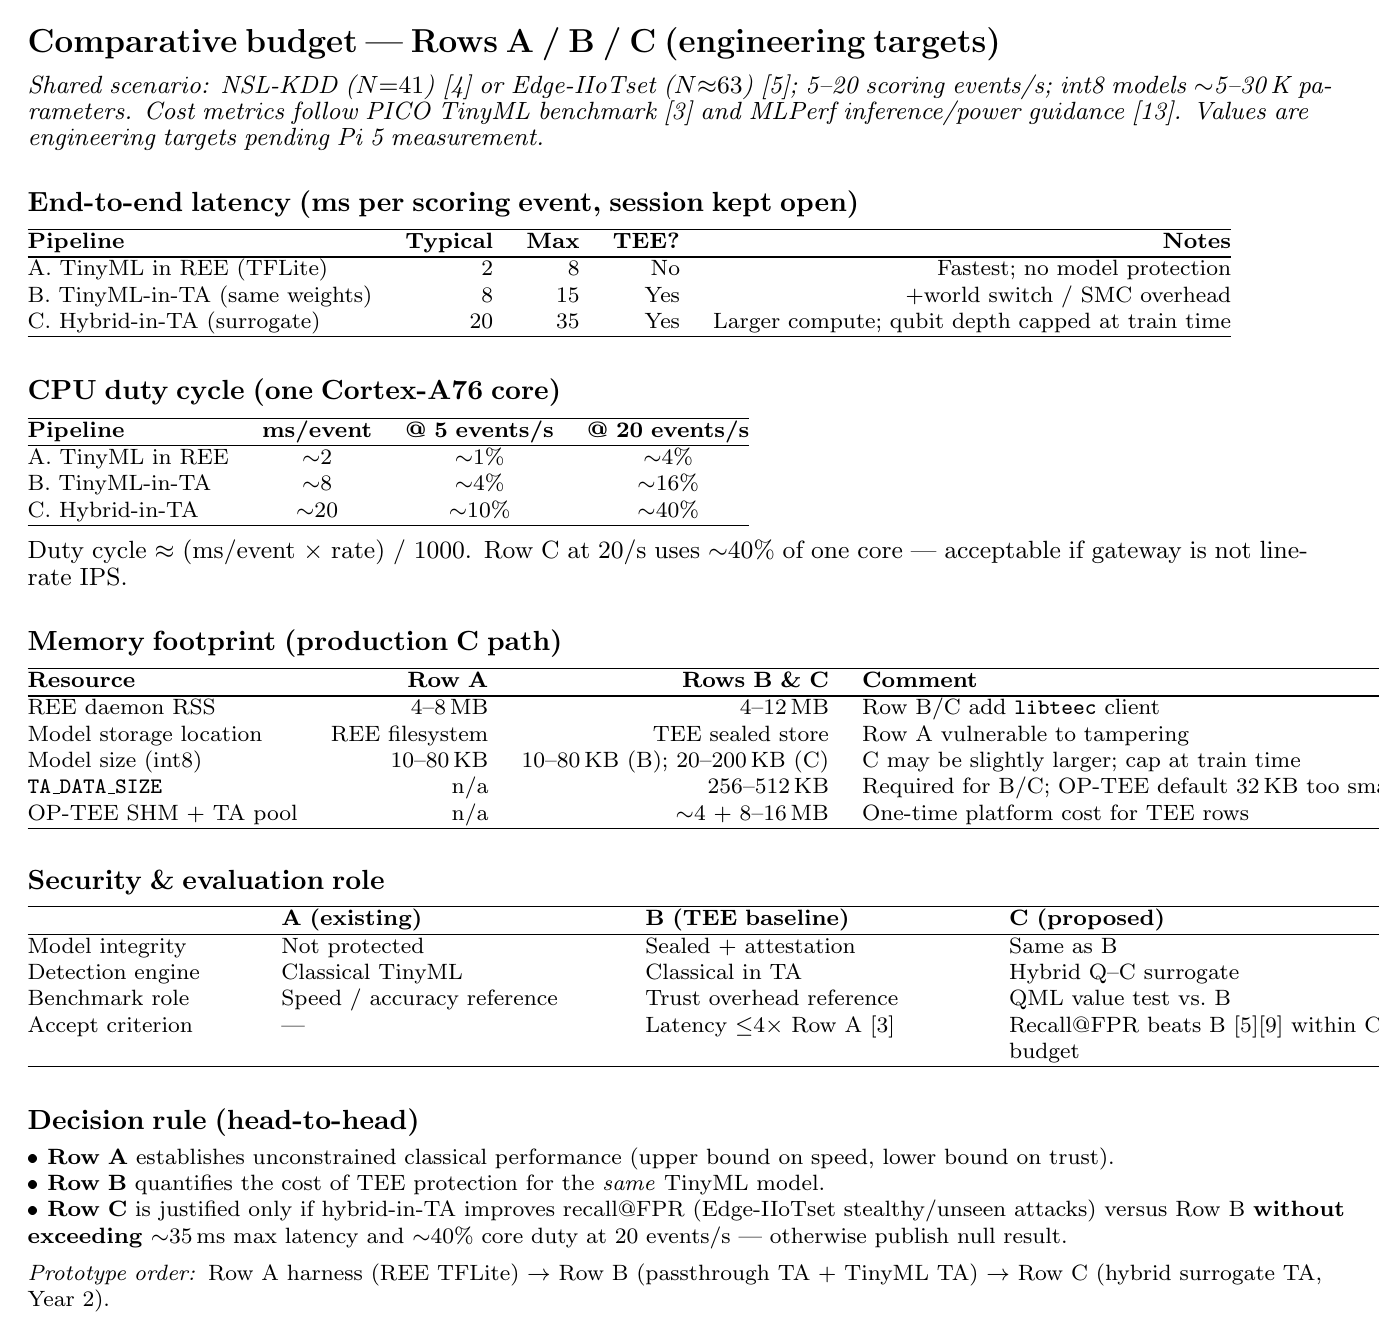
\begin{tikzpicture}
\node[qpage] at (0,0) {%
  {\bfseries\large Comparative budget --- Rows A / B / C (engineering targets)}\\[4pt]
  {\small\textit{Shared scenario: NSL-KDD ($N{=}41$) [4] or Edge-IIoTset ($N{\approx}63$) [5]; 5--20 scoring events/s; int8 models ${\sim}$5--30\,K parameters. Cost metrics follow PICO TinyML benchmark [3] and MLPerf inference/power guidance [13]. Values are engineering targets pending Pi~5 measurement.}}\\[8pt]

  \qaheading{End-to-end latency (ms per scoring event, session kept open)}
  \begin{tabular}{@{}lrrrr@{}}
    \hline
    \textbf{Pipeline} & \textbf{Typical} & \textbf{Max} & \textbf{TEE?} & \textbf{Notes} \\
    \hline
    A.\ TinyML in REE (TFLite)      & 2  & 8  & No  & Fastest; no model protection \\
    B.\ TinyML-in-TA (same weights) & 8  & 15 & Yes & +world switch / SMC overhead \\
    C.\ Hybrid-in-TA (surrogate)    & 20 & 35 & Yes & Larger compute; qubit depth capped at train time \\
    \hline
  \end{tabular}\\[8pt]

  \qaheading{CPU duty cycle (one Cortex-A76 core)}
  \begin{tabular}{@{}lccc@{}}
    \hline
    \textbf{Pipeline} & \textbf{ms/event} & \textbf{@ 5 events/s} & \textbf{@ 20 events/s} \\
    \hline
    A.\ TinyML in REE     & ${\sim}$2  & ${\sim}$1\%  & ${\sim}$4\% \\
    B.\ TinyML-in-TA      & ${\sim}$8  & ${\sim}$4\%  & ${\sim}$16\% \\
    C.\ Hybrid-in-TA      & ${\sim}$20 & ${\sim}$10\% & ${\sim}$40\% \\
    \hline
  \end{tabular}\\[4pt]
  {\small Duty cycle $\approx$ (ms/event $\times$ rate) / 1000. Row C at 20/s uses ${\sim}$40\% of one core --- acceptable if gateway is not line-rate IPS.}\\[8pt]

  \qaheading{Memory footprint (production C path)}
  \begin{tabular}{@{}lrrp{7.5cm}@{}}
    \hline
    \textbf{Resource} & \textbf{Row A} & \textbf{Rows B \& C} & \textbf{Comment} \\
    \hline
    REE daemon RSS           & 4--8\,MB   & 4--12\,MB  & Row B/C add \texttt{libteec} client \\
    Model storage location   & REE filesystem & TEE sealed store & Row A vulnerable to tampering \\
    Model size (int8)        & 10--80\,KB & 10--80\,KB (B); 20--200\,KB (C) & C may be slightly larger; cap at train time \\
    \texttt{TA\_DATA\_SIZE}  & n/a        & 256--512\,KB & Required for B/C; OP-TEE default 32\,KB too small \\
    OP-TEE SHM + TA pool     & n/a        & ${\sim}$4 + 8--16\,MB & One-time platform cost for TEE rows \\
    \hline
  \end{tabular}\\[8pt]

  \qaheading{Security \& evaluation role}
  \begin{tabular}{@{}p{2.8cm}p{4.2cm}p{4.2cm}p{4.8cm}@{}}
    \hline
    & \textbf{A (existing)} & \textbf{B (TEE baseline)} & \textbf{C (proposed)} \\
    \hline
    Model integrity   & Not protected & Sealed + attestation & Same as B \\
    Detection engine  & Classical TinyML & Classical in TA & Hybrid Q--C surrogate \\
    Benchmark role    & Speed / accuracy reference & Trust overhead reference & QML value test vs.\ B \\
    Accept criterion  & --- & Latency $\leq$4$\times$ Row A [3] & Recall@FPR beats B [5][9] within C budget \\
    \hline
  \end{tabular}\\[8pt]

  \qaheading{Decision rule (head-to-head)}
  \textbullet\ \textbf{Row A} establishes unconstrained classical performance (upper bound on speed, lower bound on trust).\\
  \textbullet\ \textbf{Row B} quantifies the cost of TEE protection for the \emph{same} TinyML model.\\
  \textbullet\ \textbf{Row C} is justified only if hybrid-in-TA improves recall@FPR (Edge-IIoTset stealthy/unseen attacks) versus Row B \textbf{without exceeding} ${\sim}$35\,ms max latency and ${\sim}$40\% core duty at 20 events/s --- otherwise publish null result.\\[4pt]
  \textit{Prototype order:} Row A harness (REE TFLite) $\rightarrow$ Row B (passthrough TA + TinyML TA) $\rightarrow$ Row C (hybrid surrogate TA, Year~2).%
};
\end{tikzpicture}

%% ---------------------------------------------------------------------------
%% Page 4 — References and cost-metric standards
%% ---------------------------------------------------------------------------
\newpage
\begin{tikzpicture}
\node[qpage, font=\scriptsize] at (0,0) {%
  {\bfseries\large References and cost-metric standards}\\[6pt]

  \qaheading{Pipeline mapping (Rows A / B / C)}
  \textbf{Row A} (TinyML in REE): TFLite Micro runtime [1], TinyML practice [2], PICO cost metrics [3], datasets [4][5].\\
  \textbf{Row B} (+ TEE): OP-TEE TA model [6][7][8], same TinyML export path as A; adds secure-world inference overhead.\\
  \textbf{Row C} (+ hybrid QML): Chowdhury \textit{et al.}\ [9], PennyLane [10], D'Amore \textit{et al.}\ [11], embedded QML feasibility [12]; builds on B with offline QML training and C surrogate in TA.\\[8pt]

  \qaheading{Standard cost and evaluation metrics (this study)}
  \begin{tabular}{@{}p{3.2cm}p{5.5cm}p{7.3cm}@{}}
    \hline
    \textbf{Metric} & \textbf{Definition / target} & \textbf{Standard / reference} \\
    \hline
    Inference latency   & Wall-clock ms per scoring event (session open) & PICO-tinyML-benchmark [3]; \texttt{clock\_gettime} \\
    End-to-end latency  & Ingest $\rightarrow$ alert; target $\leq$100\,ms & Edge IDS SLA practice [5] \\
    CPU duty cycle      & (\texttt{ms/event} $\times$ rate) / 1000 on one core & PICO CPU utilization [3] \\
    REE RSS memory      & CA + buffers (MB) & \texttt{/proc/self/status}; PICO memory efficiency [3] \\
    TA heap / stack     & \texttt{TA\_DATA\_SIZE}, \texttt{TA\_STACK\_SIZE} & OP-TEE TA properties [6][7] \\
    Model size          & Sealed int8 weights (KB) & TinyML compression [1][2] \\
    Energy / inference  & Joules or mJ per scored flow & MLPerf power methodology [13] \\
    Detection quality   & Recall@FPR (e.g.\ 1\%), AUC, F1 & Edge-IIoTset IDS evaluation [5]; family hold-out for unseen attacks \\
    Trust overhead      & B vs A latency ratio ($\leq$4$\times$ target) & TEE SMC + TA invoke [6][8] \\
    \hline
  \end{tabular}\\[10pt]

  \qaheading{Reference list}
  \begin{enumerate}
    \setlength{\itemsep}{2pt}
    \item R.~David \textit{et al.}, ``TensorFlow Lite Micro: Embedded Machine Learning on TinyML Systems,'' \textit{Proc.\ MLSys}, 2021. \textit{(Row A runtime --- TFLite Micro / edge inference.)}
    \item P.~Warden and D.~Situnayake, \textit{TinyML: Machine Learning with TensorFlow Lite on Arduino and Ultra-Low-Power Microcontrollers}. O'Reilly, 2019. \textit{(Row A TinyML workflow: train, quantize, deploy.)}
    \item A.~Dey, S.~Srivastava, G.~Singh, and R.~G.~Pettit, ``Real-Time Performance Benchmarking of TinyML Models in Embedded Systems (PICO),'' arXiv:2509.04721, 2025. \textit{(Latency, CPU, memory, stability metrics.)}
    \item M.~Tavallaee, E.~Bagheri, W.~Lu, and A.~A.~Ghorbani, ``A Detailed Analysis of the KDD CUP 99 Data Set,'' \textit{Proc.\ IEEE CISDA}, 2009. DOI: 10.1109/CISDA.2009.5356528. \textit{(NSL-KDD dataset.)}
    \item M.~A.~Ferrag \textit{et al.}, ``Edge-IIoTset: A New Comprehensive Realistic Cyber Security Dataset of IoT and IIoT Applications,'' \textit{IEEE Access}, vol.~10, pp.~40281--40306, 2022. DOI: 10.1109/ACCESS.2022.3165809. \textit{(Primary IIoT IDS dataset; recall@FPR evaluation.)}
    \item OP-TEE Documentation, ``Trusted Applications,'' OP-TEE v4.x. \url{https://optee.readthedocs.io/en/latest/building/trusted_applications.html}. \textit{(\texttt{TA\_DATA\_SIZE}, \texttt{TA\_STACK\_SIZE}; Row B/C TA build.)}
    \item OP-TEE Documentation, ``Trusted Applications Architecture,'' OP-TEE v4.x. \url{https://optee.readthedocs.io/en/latest/architecture/trusted_applications.html}. \textit{(TEE Internal Core API, \texttt{TEE\_InvokeCommand}.)}
    \item Linaro SWG, ``TA Properties Basics,'' \textit{optee\_examples} docs. \url{https://github.com/linaro-swg/optee_examples}. \textit{(Row B passthrough / inference TA; libteec client.)}
    \item S.~Chowdhury \textit{et al.}, ``Quantum Machine Learning for Anomaly Detection in IoT Devices,'' \textit{Proc.\ AIMLSystems (Quantum Symposium)}, 2025. \textit{(Row C QML-for-IoT-IDS prior art.)}
    \item V.~Bergholm \textit{et al.}, ``PennyLane: Automatic differentiation of hybrid quantum-classical computation,'' \textit{Advances in Quantum Technologies}, 2022. \textit{(Hybrid training toolchain --- offline only.)}
    \item F.~D'Amore \textit{et al.}, ``Projected Quantum Kernel for IoT Data Analysis,'' \textit{Proc.\ IEEE PICom}, pp.~200--204, 2024. DOI: 10.1109/PICom64201.2024.00032. \textit{(Quantum-kernel IoT classification; cloud/simulator baseline.)}
    \item A.~Dey and K.~Raza, ``Embedded Quantum Machine Learning: Feasibility and Hybrid Architectures,'' 2026. \textit{(Edge QML deployability evidence gap cited in doctoral survey.)}
    \item MLCommons, ``MLPerf Inference Benchmark Rules,'' v4.x; ``MLPerf Power Measurement,'' MLCommons, 2023--2024. \url{https://mlcommons.org/en/inference/}. \textit{(Joules/inference and standardized power reporting.)}
  \end{enumerate}%
};
\end{tikzpicture}
\end{document}
